%\documentclass[a4paper,handout]{beamer}
\documentclass[presentation]{beamer}
%\usepackage[francais]{babel}
\usepackage[utf8]{inputenc}
\usetheme{Inuits}
\usepackage[T1]{fontenc}
\usepackage{listings}
\usepackage{eso-pic}
\setbeamercolor{background canvas}{bg=}
\definecolor{inuitstitle}{RGB}{153,153,255}
\definecolor{inuitsgreen}{RGB}{35,255,35}
\usecolortheme[RGB={90,90,149}]{structure}
\usebackgroundtemplate{%
\includegraphics[height=\paperheight,width=\paperwidth]{files/background.png};}

%\AddToShipoutPicture{\put(0,5){%
%   \parbox[b][\paperheight]{\paperwidth}{%
%     \vfill
%     \centering
%     \rotatebox{0}{\includegraphics[width=\paperwidth,height=\paperheight,%
%                      ]{files/background.png}}%
%     \vfill
%}}}
\setbeamercolor{normal text}{fg=white}
\setbeamercolor{block body}{fg=black}
\setbeamercolor{itemize item}{fg=inuitsgreen}
\setbeamercolor{itemize subitem}{fg=inuitsgreen}
\setbeamercolor{itemize subitem subitem}{fg=inuitsgreen}
\setbeamertemplate{itemize item}[circle]
\setbeamertemplate{itemize subitem}[circle]
\setbeamertemplate{sections/subsections in toc}[circle]

%\setbeamercolor{palette primary}{fg=inuitstitle,bg=black!85}
%\setbeamercolor{palette secondary}{fg=white,bg=inuitstitle}
%\setbeamercolor{palette tertiary}{fg=white,bg=black!85}
%\setbeamercolor{palette quaternary}{fg=inuitstitle}
%\setbeamercolor{block title}{fg=inuitstitle}
%\setbeamercolor{sidebar}{bg=inuitstitle!70}

%\AtBeginDocument{%
%    \pgfdeclareverticalshading{beamer@topshade}{\paperwidth}{%
%      color(0pt)=(bg);
%      color(4pt)=(black)}
%}


\setbeamercolor{title}{fg=inuitstitle,bg=}

\setbeamertemplate{navigation symbols}{}
\definecolor{OliveGreen}{RGB}{0,100,0}
\definecolor{grey}{RGB}{150,150,150}
\definecolor{darkgrey}{RGB}{100,100,100}
\definecolor{inuits}{RGB}{153,153,255}
\usepackage{shadowtext}

\usepackage{pdfpages}
\newcommand{\xitem}[1]{\item{\shadowtext{#1}}}
\newcommand{\inuits}[1]{\shadowtext{\color{inuits}#1}}
\newcommand{\RelatedText}[4][0.65\textwidth]{%
\begin{math}%
  \left.% 
    \parbox{#1}{#3}\vphantom{\parbox{#1}{#4}}%
     \right#2%
      \parbox{#1}{#4}\vphantom{\parbox{#1}{#3}}%
     \end{math}
    }%

\newcommand{\ptitle}{Building and Deploying Mediasalsa}

\begin{document}
\setbeamercovered{invisible}
\title[\ptitle]{\fontsize{20}{35}\selectfont \shadowtext{\ptitle}}
\subtitle{\shadowtext{A Drupal Digital Asset Management system as a Service}}

\author[Julien Pivotto]{\shadowtext{Julien Pivotto}}
%\institute[Inuits]{Inuits}
\date{\shadowtext{DrupalCon Prague}\\\inuits{September 26, 2013}}
\logo{
\includegraphics[height=1cm]{files/logo-prague.png}}

\frame[plain,t]{\vspace{-1em} \centerline{\includegraphics[width=\paperwidth]{files/loup.jpg}}\titlepage}
%\frame{\tableofcontents}
\begin{frame}
\frametitle{MediaMosa}
    \begin{center}
        
\includegraphics[height=3cm]{files/mediamosa.png}\\
    \end{center}
\begin{itemize}
\xitem{Drupal-based Digital Asset Management system}
\xitem{Open-source}
\xitem{Store assets}
\xitem{Trancode videos}
\item{\shadowtext{Create, extract and manage metadata using open standards:}\\
\shadowtext{Dublin Core, Qualified DC, IEEE/LOM, CZP}}
\xitem{Webservice oriented}
\end{itemize}
\end{frame}
\begin{frame}
\frametitle{MediaSalsa}
    \begin{center}
        
\includegraphics[height=2cm]{files/mediasalsa.png}\\
        \Huge{\shadowtext{$=$}}\\
        \Huge{\shadowtext{MediaMosa as a Service}}
    \end{center}
\end{frame}
\begin{frame}
\frametitle{MediaSalsa infrastructure (simplified)}
\RelatedText{\}}{%
\begin{itemize}
\xitem{Backend: Core service (MediaMosa)}
\xitem{Frontends: Optional}
\xitem{Web servers}
\xitem{Database server}
\xitem{Solr server}
\xitem{Transcoding servers}
\end{itemize}
}{\shadowtext{for each environment}}
\end{frame}
%\section{Culture}
\frame{%
\begin{center}
\Huge{\color{inuits}Culture}\\
\LARGE{\color{grey}Automation}\\
\LARGE{\color{grey}Measurement}\\
\LARGE{\color{grey}Sharing}
\end{center}
}
%\subsection{Our company}
\begin{frame}
\frametitle{Inuits}
\begin{itemize}
\LARGE
\xitem{Inuits is an {\color{inuits}Open-Source} company}
\begin{itemize}
\LARGE
\item[$\Rightarrow$]{\shadowtext{We contribute back}}
\end{itemize}
\xitem{$\pm$ 40 people in 3 countries}
\xitem{One language: English}
\end{itemize}
\end{frame}
\begin{frame}
\frametitle{Inuits}
\begin{center}
\large
What do we do?
\end{center}
\begin{itemize}
\LARGE
\xitem{Consulting {\color{inuits}and} Internal projects}
\xitem{Development {\color{inuits}and} System administration}
\end{itemize}
\end{frame}
\begin{frame}
\frametitle{Inuits}
\begin{center}
\LARGE
\shadowtext{Ideal world {\color{red}vs} budget and reality}\\
\LARGE
\shadowtext{$\Rightarrow$ pragmatic approach}
\end{center}
\end{frame}
%\subsection{The teams}
\begin{frame}
\frametitle{Distributed team}
\begin{center}
\Huge{Communication $=$ \color{red}hell}\\
%find a nice picture
\vspace{0.7cm}
\LARGE How to fix it?
\end{center}
\begin{itemize}
\xitem{Daily virtual stand-up over XMPP/Hangout}
\xitem{Redmine project managment}
\begin{itemize}
\xitem{Tasks}
\xitem{Repositories}
\xitem{Documentation (wiki)}
\end{itemize}
\xitem{Internal mailing lists}
\xitem{Jenkins notifications by mail and XMPP}
\xitem{Internal training}
\end{itemize}
\end{frame}
\begin{frame}
\frametitle{Dev and Ops}
\begin{columns}[t]
\column{.5\textwidth}
\center{\Huge \shadowtext{Dev}}\\
\begin{itemize}
\xitem{Develop new features}
\xitem{Write tests}
\end{itemize}
\column{.5\textwidth}
\center{\Huge \shadowtext{Ops}}\\
\begin{itemize}
\xitem{Infrastructure (puppet)}
\xitem{CD and CI (jenkins)}
\end{itemize}
\end{columns}
\begin{center}
\shadowtext{Ops teach dev to think about {\color{inuits}monitoring} and {\color{inuits}distributed service}}\\
\shadowtext{Dev teach to ops about required libraries and tests}
\end{center}
\end{frame}




%\section{Automation}
\frame{%
\begin{center}
\LARGE{\color{grey}Culture}\\
\Huge{\color{inuits}Automation}\\
\LARGE{\color{grey}Measurement}\\
\LARGE{\color{grey}Sharing}
\end{center}
}
%\subsection{Puppet}
\begin{frame}
\frametitle{Puppet}
\begin{center}
\LARGE {\color{inuits}Puppet} automates {\color{inuits} all the things}\\
\vspace{1cm}
\large {$\Rightarrow$\hspace{0.3cm}\color{inuits}mcollective} orchestrates {\color{inuits} all the things}
\end{center}
\end{frame}
\begin{frame}
\frametitle{CD}
\begin{center}
\large
\shadowtext{Continuous Delivery {\color{red}vs} Continuous Deployment}
\end{center}
\begin{itemize}
\xitem{Puppet code}
\begin{itemize}
\xitem{Deployed to dev environment}
\xitem{Same puppet code for each environment}
\xitem{User-triggered deployments to UAT and prod}
\xitem{Feature flags in Puppet code per environment}
\end{itemize}
\xitem{Application code}
\begin{itemize}
\xitem{Continuous integration in dev}
\xitem{User-triggered deployments to UAT}
\xitem{Deployment to prod is a business decision}
\end{itemize}
\end{itemize}
\end{frame}
%\subsection{Jenkins}
\begin{frame}
\frametitle{Tests}
\begin{center}
\LARGE{Developers test a lot}
\end{center}
\begin{itemize}
\item[\dots]{\shadowtext{The tests don't work}}
\item[\dots]{\shadowtext{It works on my machine}}
\item[\dots]{\shadowtext{Wrong platform}}
\item[\dots]{\shadowtext{Wrong PHP version}}
\item[$\Rightarrow$]{\large\shadowtext{\color{green}Fixed now, thanks to Jenkins!}}
\end{itemize}
%\begin{right}
\end{frame}
%\begin{frame}
%\frametitle{Environments}
%\RelatedText{\}}{%
%\begin{itemize}
%\xitem{Development}
%\xitem{UAT}
%\xitem{Prod}
%\begin{itemize}
%\xitem{.ac}
%\xitem{.com}
%\xitem{dedicated}
%\end{itemize}
%\end{itemize}}{\shadowtext{$\neq$ versions}}
%\end{frame}
\begin{frame}
\frametitle{SCM}
\begin{center}
{\huge
\shadowtext{Code is under revision control (git)}
}
\large
\begin{itemize}
\xitem{Prefer small commits}
\xitem{Local features branches}
\xitem{Packages}
\end{itemize}
\end{center}
\end{frame}
\begin{frame}
\frametitle{Using OS packaging system}
\begin{itemize}
\xitem{Consistency, security, dependencies}
\xitem{Uniquely identify where files are coming from}
\xitem{Source repo may not be reacheable}
\xitem{Little overhead when you automate}
\xitem{\color{red}Configuration does not belong to a package}
\end{itemize}
\end{frame}
\begin{frame}
\frametitle{Pipelines}
\begin{itemize}
\xitem{A collection of jobs}
\xitem{Run one after another}
\xitem{Start on checkout, end on deployment}
\xitem{From the developers' side:}
\begin{itemize}
\item[$\Rightarrow$]{\shadowtext{Git push}}
\item[$\Leftarrow$]{\shadowtext{Mail with changes + link to deploy}}
\end{itemize}
\end{itemize}
\end{frame}
\begin{frame}[fragile]
\frametitle{Our pipelines}
\begin{itemize}
\xitem{Puppetized}
\xitem{Puppet code and Application code (backend and frontends)}
\xitem{1 pipeline/project/customer}
\vspace{0.5cm}
\begin{block}{Defining a pipeline}
\footnotesize
\texttt{salsajobs::pipeline::frontend~\{}\\
\texttt{~'qwerty-inc':}\\
\texttt{~~git\_repository~=>~'ssh://git@redmine/qwerty.git',}\\
\texttt{~~dashboard\_view~=>~'mds-frontends',}\\
\texttt{~~target\_urls~~~~=>~\{}\\
\texttt{~~~~'uat'~~~~~~~~=>~'http://qwerty.uat.mediasalsa.eu',}\\
\texttt{~~~~'prod'~~~~~~~=>~'http://qwerty.mediasalsa.eu',}\\
\texttt{~~\},}\\
\texttt{~~require~~~~~~~~=>~Salsajobs::Views::Dashboard['mds-frontends'],}\\
\texttt{\}}
\end{block}
\end{itemize}
\end{frame}
\begin{frame}
\frametitle{Pipelines steps}
    \begin{center}
        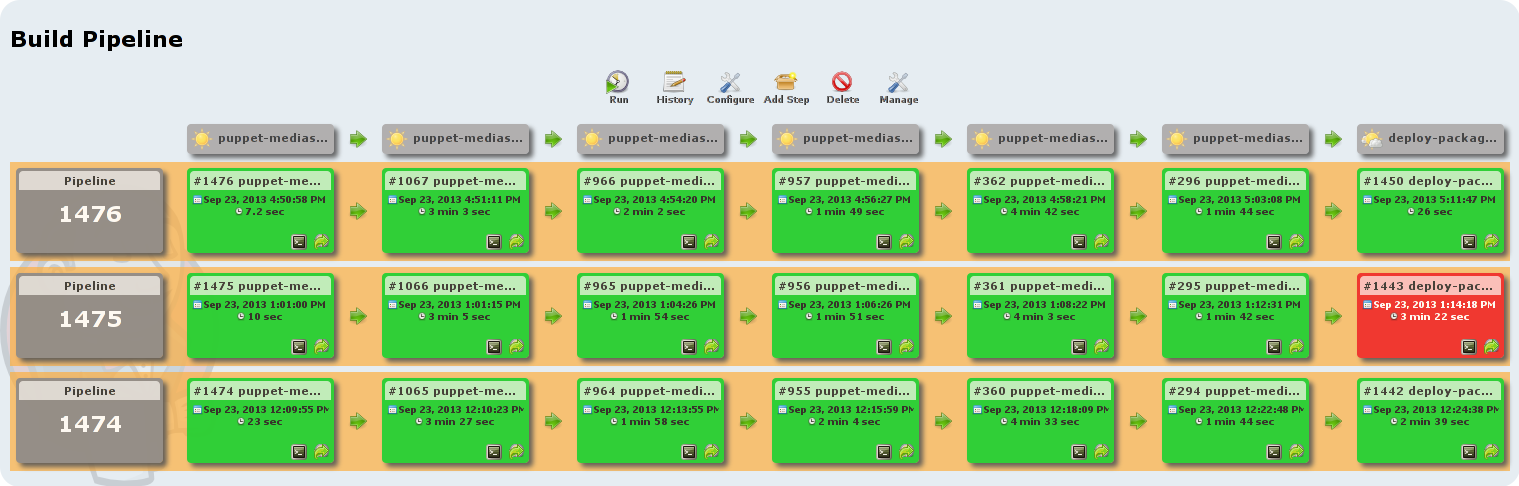
\includegraphics[width=10cm]{files/pipeline-drupalcon.png}\\
    \end{center}
\begin{itemize}
\xitem{Checkout}
\xitem{Syntax: \texttt{php -l}}
\xitem{Style: Drupal Coder}
\xitem{Package: FPM}
\xitem{Deploy to dev environment: Mco}
\xitem{Tests in dev environment: \texttt{drush run-tests}}
\xitem{Publish package and promote: Mco}
\end{itemize}
\end{frame}
\begin{frame}
\frametitle{Promotion}
    \begin{center}
        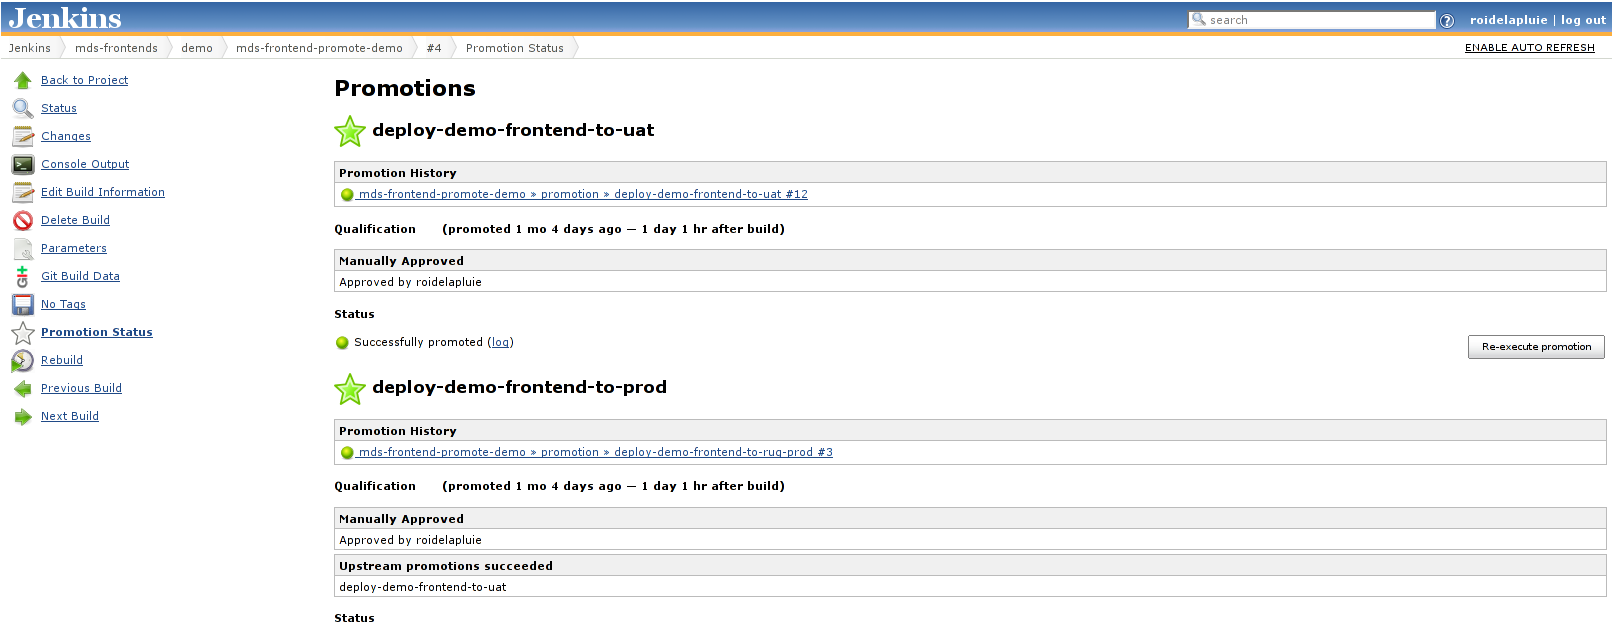
\includegraphics[width=11cm]{files/promotion.png}\\
    \end{center}
\begin{itemize}
\xitem{At the end of the pipeline}
\xitem{Send a simple email}
\begin{itemize}
\xitem{A link to the promotion page}
\xitem{The changelog}
\end{itemize}
\xitem{Promotion page contains one button per environment}
\xitem{Must promote to UAT before Production}
\end{itemize}
\end{frame}
\begin{frame}
\frametitle{Tools used with jenkins}
\begin{itemize}
%TODO: add drush php tests, etc
\xitem{Pulp to manage RPM repositories}
\xitem{Mcollective to update packages, run drush}
\end{itemize}
\end{frame}









%\section{Measurement}
\frame{%
\begin{center}
\LARGE{\color{grey}Culture}\\
\LARGE{\color{grey}Automation}\\
\Huge{\color{inuits}Measurement}\\
\LARGE{\color{grey}Sharing}
\end{center}
}
\begin{frame}
\frametitle{Logstash}
\begin{center}
\huge
Collect all the logs
\end{center}
\begin{itemize}
\xitem{Drupal logs}
\xitem{Apache logs}
\xitem{Deployment logs}
\xitem{System logs}
\item[$\Rightarrow$]{\color{green}\shadowtext{Logstash, ES, kibana, statsd, graphite}}
\end{itemize}
\end{frame}
\begin{frame}
\frametitle{Icinga}
\begin{center}
\huge
Monitor everything
\end{center}
\begin{itemize}
\xitem{"Basics"}
\item[$+$]{\shadowtext{vhosts}}
\item[$+$]{\shadowtext{databases}}
\item[$+$]{\shadowtext{cronjobs}}
\end{itemize}
\end{frame}
\begin{frame}
\frametitle{Graphite + gdash}
\begin{itemize}
\xitem{Collectd}
\xitem{Monitor platform usage}
\xitem{FFmpeg usage}
\xitem{Number of accounts (backend ID's)}
\end{itemize}
\end{frame}
\begin{frame}
\frametitle{FFmpeg}

    \begin{center}
        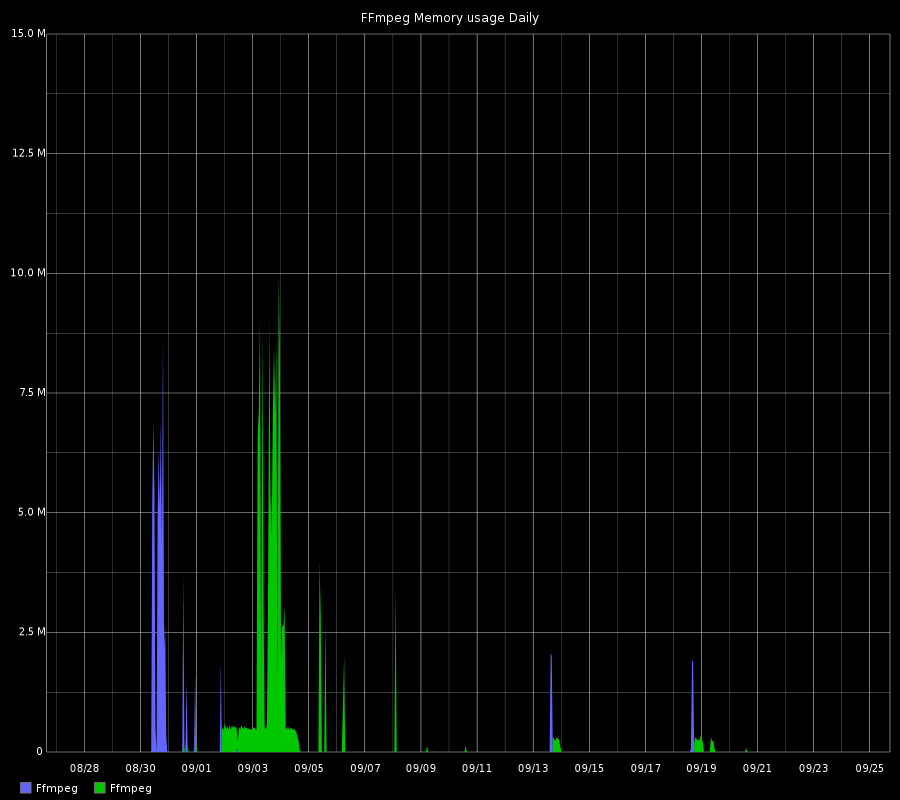
\includegraphics[height=8cm]{files/ffmpeg.png}\\
    \end{center}
\end{frame}

\begin{frame}
\frametitle{Managed assets}

    \begin{center}
        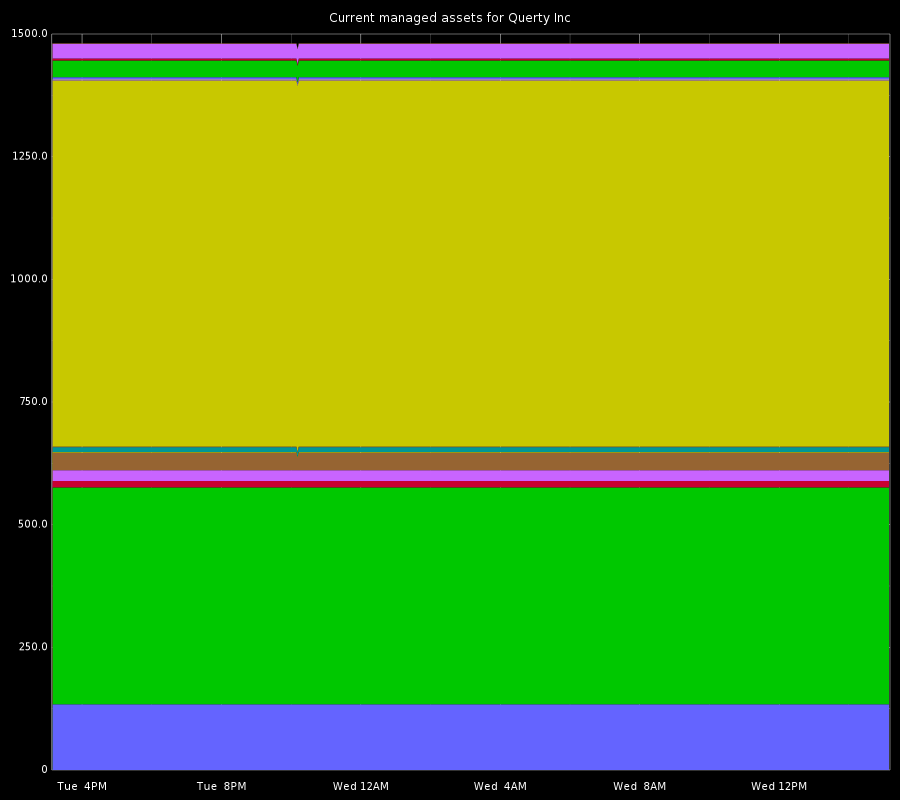
\includegraphics[height=8cm]{files/managed.png}\\
    \end{center}
\end{frame}

\begin{frame}
\frametitle{Number of backend ID's}

    \begin{center}
        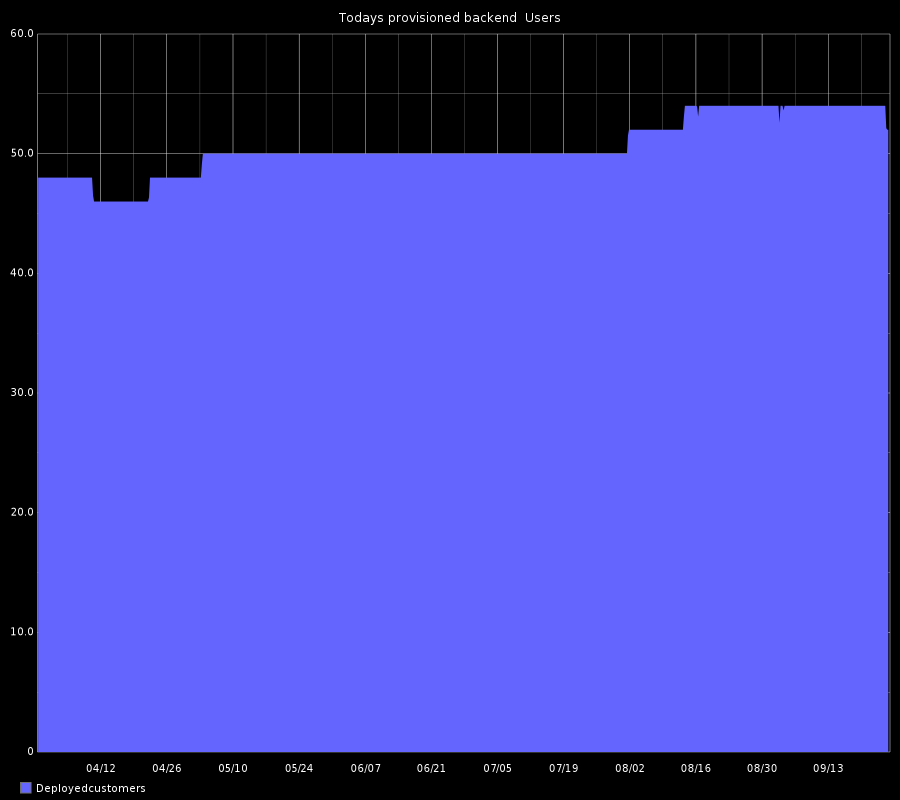
\includegraphics[height=8cm]{files/graphite.png}\\
    \end{center}
\end{frame}






%\section{Sharing}
\frame{%
\begin{center}
\LARGE{\color{grey}Culture}\\
\LARGE{\color{grey}Automation}\\
\LARGE{\color{grey}Measurement}\\
\Huge{\color{inuits}Sharing}
\end{center}
}
\begin{frame}
\frametitle{Sharing}
\begin{center}
\LARGE
\shadowtext{We have just {\color{inuits}\Huge{shared}} our experience\dots}\\
\vspace{2cm}
\shadowtext{Any question?}
\end{center}
\end{frame}
\frame{%
\frametitle{Contact}
    \begin{columns}[T]
        \begin{column}{.5\textwidth}
    \begin{large}
    \shadowtext{Julien Pivotto}\\
    \shadowtext{julien@inuits.eu}\\
    \shadowtext{@roidelapluie}
    \end{large}
        \end{column}
        \begin{column}{.5\textwidth}
    \vspace{2cm}
    \begin{small}
    \includegraphics[height=2cm]{files/inuitslogo.png}\\
    \shadowtext{INUITS bvba}\\
    \shadowtext{Duboisstraat 50}\\
    \shadowtext{2060 Antwerp}\\
    \shadowtext{Belgium}\\
    \shadowtext{+32 473 441 636}\\
    \shadowtext{https://inuits.eu}
    \end{small}
        \end{column}
        \end{columns}
}
{%
\usebackgroundtemplate{}
\setbeamercolor{background canvas}{bg=}

\includepdf{slides.pdf}
}



%\begin{frame}
%\frametitle{}
%\begin{itemize}
%\xitem{}
%\end{itemize}
%\end{frame}
%\begin{frame}
%\frametitle{}
%\begin{itemize}
%\xitem{}
%\end{itemize}
%\end{frame}
%\begin{frame}
%\frametitle{}
%\begin{itemize}
%\xitem{}
%\end{itemize}
%\end{frame}
%\begin{frame}
%\frametitle{}
%\begin{itemize}
%\xitem{}
%\end{itemize}
%\end{frame}

\end{document}
